\chapter{Descripción de la Solución}

A continuación se describe la solución propuesta con motivo de este trabajo de memoria, partiendo de conceptos más teóricos para luego abordar algunos temas de decisiones de implementación y mostrar el resultado final de la aplicación que se desarrolló.

\section{SNM, Social Network Model} % (fold)
\label{sec:snm_social_network_model}

Uno de los puntos principales de esta memoria, es poner en práctica el modelo realizado por el alumno de doctorado en el DCC, Mauro San Martín\cite{tesismauro}, quien investigó y propuso un modelo llamado \emph{Social Network Model} o SNM. Por lo tanto, la generación de redes sociales en esta aplicación tendrán en cuenta este modelo, trabajo que fue guiado por el mismo profesor guía de esta memoria, aprovechando la experiencia e investigación previa sobre el tema. Entonces, se procederá a definir y explicar brevemente en que consiste este modelo.

\subsection{Elementos de Redes Sociales} % (fold)
\label{sub:elementos_de_redes_sociales}

Para el modelo de Mauro se tienen algunos elementos pertenecientes a las redes sociales, que fueron tratados en los conceptos de redes sociales en la sección \ref{sec:conceptos_de_redes_sociales}, a los cuales se les agregan algunas restricciones:

  \begin{itemize}
    \item Los \emph{Actores}: estos tienen un identificador único y un conjunto de atributos, además pueden participar en cualquier número de relaciones.
    \item Las \emph{Relaciones} también tiene un identificador único, un conjunto de atributos y un número de actores participantes. El número de participantes puede ser uno o más, y puede cambiar sin afectar el resto de las propiedades de la relación.
    \item Los \emph{Atributos} tienen un significado asociado y un valor literal. Un atributo es identificado por el identificador del objeto al cual está añadido (acto o relación), por su significado y su valor literal. La clase de un objeto (actor o relación) es un tipo de atributo especial llamado \emph{familia}.
    \item \emph{Actores}, \emph{Relaciones}, \emph{Atributos} y sus conexiones forman una red social. Compartiendo y reusando metadata al nivel, por ejemplo, proveniencia de conjuntos de datos.
  \end{itemize}

\subsection{Definición Matemática} % (fold)
\label{sub:definicion_matematica}

Dado lo anterior, el modelo \emph{SNM} describe una red social como un grafo de la siguiente forma:

\begin{defn}
  (Red Social Generalizada) Una red social generalizada es definida como un multigrafo dirigido tripartito con etiquetas junto con una familia de funciones equitetadoras $f$ y un conjunto de familia de etiquetas $L_f$:
  
  \begin{center}
    $ G = (N, E, L_N, L_E, L_f, \iota, \nu, \epsilon, f) $
  \end{center}
  
  Donde:
  
  \begin{itemize}
    \item El conjunto de nodos $N = A \cup T \cup C$ es una unión disjunta del conjunto de actores $A$, con el conjunto de relaciones $T$ y el conjunto de atributos $C$.
    \item Existe una colección finita de familias (subconjuntos) de actores $\mathcal{A} = \{ A_1, A_2, \dotsc, A_k \}$ de manera tal que cada $A_i \subseteq A$ y $\cup_{1 \leq i \leq k}A_i = A$.
    \item Donde existe una colección finita de familias (subconjuntos) de relaciones $\mathcal{T} = \{ T_1, T_2, \dotsc, T_j \}$ donde cada $T_i \subseteq T$ y $\cup_{1 \leq i \leq k}T_i = T$.
    \item El conjunto de arcos $E = E_{AT} \cup E_{AC} \cup E_{TC}$ es la unión disjunta del conjunto de arcos entre actores y relaciones $E_{AT}$, con el conjunto de arcos entre actores y atributos $E_{AC}$, el conjunto de arcos entre atributos y relaciones $E_{TC}$.
    \item El conjunto de etiquetas de nodo $L_N = L_A \cup L_T \cup L_C$ es la unión disjunta de los conjuntos de etiquetas de actores $L_A$, de etiquetas de relaciones $L_T$ y el de etiquetas de atributos $L_C$.
    \item El conjunto de etiquetas de arcos $L_E = L_{AT} \cup L_{AC} \cup L_{TC}$ es la unión disjunta de los conjuntos de etiquetas de arcos entre actores y relaciones $L_{AT}$ (roles de participación), de etiquetas de arcos entre actores y atributos $L_{AC}$ (significado de atributos de actores) y el de etiquetas de arcos entre relaciones y atributos $L_{TC}$ (significado de atributos de relaciones).
    \item El conjunto de etiquetas de familias $L_f = L_{f_A} \cup L_{f_T}$ es la unión disjunta entre el conjunto de etiquetas de familias de actores $L_{f_A}$ y el conjunto de etiquetas de familias de relaciones $L_{f_T}$.
    \item $\iota = \{ \iota_{AT} , \iota_{AC} , \iota_{TC} \}$ es el conjunto de funciones de incidencia tales que $ \iota_{AT} : E_{AT} \longrightarrow A \times T$ es una función de incidencia que asocia cada arco de participación a un actor y su relación; $ \iota_{AC} : E_{AC} \longrightarrow A \times C$ es una función de incidencia que asocia un arco de significado a un actor y a un atributo; $ \iota_{TC} : E_{TC} \longrightarrow T \times C$ es una función de incidencia que asocia cada arco de significado a una relación y un atributo.
    \item $\nu = \{ \nu_A , \nu_T , \nu_C \}$ es un conjunto de funciones etiquetadoras de nodos tales que $ \nu_A : A \longrightarrow L_A$ es una función biyectiva desde actores a las etiquetas de actores; $ \nu_T : T \longrightarrow L_T$ es una función biyectiva desde relaciones a las etiquetas de las relaciones; $ \nu_C : C \longrightarrow L_C$ es una función biyectiva desde atributos a las etiquetas de atributos.
    \item $\epsilon = \{ \epsilon_{AT} , \epsilon_{AC} , \epsilon_{TC} \}$ es el conjunto de funciones etiquetadoras de arcos tales que $ \epsilon_{AT} : E_{AT} \longrightarrow L_{AT}$ es una función desde arcos de participación a sus etiquetas; $ \epsilon_{AC} : E_{AC} \longrightarrow L_{AC}$ y $ \epsilon_{TC} : E_{TC} \longrightarrow L_{TC}$ son funciones desde arcos de significado a sus etiquetas.
    \item $f = \{f_A, f_T\}$ es el conjunto de funciones etiquetadoras de familias tal que $f_A : \mathcal{A} \longrightarrow L_{f_A}$ es una función de familias de actores a las etiquetas de familias de actores y $f_T = \mathcal{T} \longrightarrow L_{f_T}$ es una función de familias de relaciones a las etiquetas de familias de relaciones.
    \item La siguiente condición se mantiene para todos los arcos entre el mismo par de actores y relaciones, Para todo $e_1$ y $e_2$ de manera tal que $\iota(e_1) = \iota(e_2) = (u,v)$ con $u \in A$ y $v \in T, e_1, e_2 \in E \Leftrightarrow \epsilon(e_1) \neq \epsilon(e_2)$.
    \item Cada función de etiquetado en $\nu, \epsilon$ y $f$, excepto $\nu_C$, deben ser invertibles.
    \item Para una relación $r \in T$ entre dos actores $a_1, a_2 \in A$, tal que existe $e_1, e_2 \in E$, y $\iota(e_1) = (a_1, r), \iota(e_2) = (a_2, r)$ con etiquetas $\epsilon(e_1) = p_1, \epsilon(e_2) = p_2$. La dirección de $r$ puede ser especificada por el par ordenado de las etiquetas de participación, eso es que una dirección $(p_1, p_2)$ indica que $r$ comienza en $a_1$ y termina en $a_2$, la dirección opuesta es representada por $(p_2, p_1)$.
  \end{itemize}
\end{defn}

De lo anterior se extrae información relevante sobre las características de las redes sociales y sus elementos:

\begin{itemize}
  \item Un \textbf{Nodo} puede ser un \emph{Actor}, \emph{Relación} o \emph{Atributo}.
  \item Las relaciones pueden ser de uno a múltiples actores.
  \item Los actores juegan un \textbf{Rol} en la relación.
  \item Los \emph{Actores} y \emph{Relaciones} pertenecen a \textbf{Familias de Actores} y \textbf{Familias de Relaciones} respectivamente.
  \item Una \textbf{Familia} de relación o actor, define un conjunto de actores/relaciones en común.
\end{itemize}

% subsection definición_matemática (end)

\subsection{Representación Gráfica} % (fold)
\label{sub:representacian_grafica}

En su tesis de doctorado\cite{tesismauro}, Mauro define un lenguaje gráfico para representar redes sociales con su modelo, el cual se adjunta a continuación por motivos de completitud del trabajo y expresar como este modelo influye posteriormente el diseño de la interfaz del usuario.\\

\begin{figure}[H]
  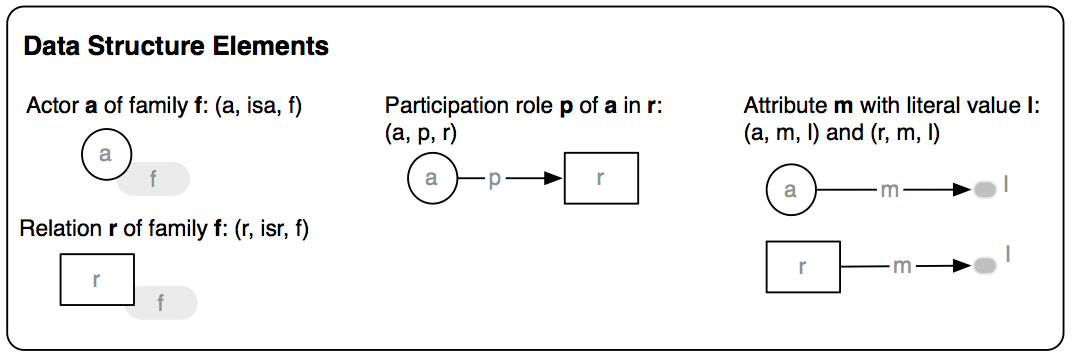
\includegraphics[width=1.0\textwidth]{images/elementos_modelo_mauro.png}
  \caption[Elementos Gráficos SNM]{\emph{Elementos Gráficos SNM}. Desde izquierda a derecha, los 4 bloques de construcción gráfica de una red social: un actor (arriba) y su etiqueta de familia, una relación y su etiqueta de familia, un rol de participación de un actor en una relación y atributos sobre actores y relaciones. Además por cada bloque se muestra la equivalencia en forma de triple.}
  \label{elementos_graficos_snm}
\end{figure}

Dados estos elementos gráficos podemos modelar una red de ejemplo como:

\begin{figure}[H]
  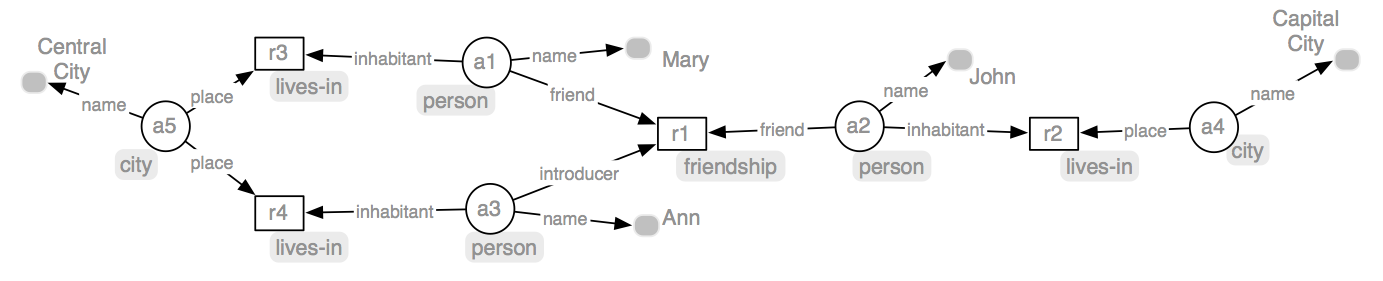
\includegraphics[width=1.0\textwidth]{images/ejemplo_red_social_mauro.png}
  \caption[Ejemplo Red Social de Amistad en SNM]{\emph{Ejemplo Red Social de Amistad en SNM}. Una red social representando relaciones de amistad (nodos cuadrados) entre Mary y John, quienes fueron presentados por Ann (los actores se muestran como nodos circulares y sus atributos como puntos grises). Las ciudades de residencia también son representadas como actores.}
  \label{ejemplo_red_snm}
\end{figure}

% subsection representación_gráfica (end)

\subsection{Representación Como Triples} % (fold)
\label{sub:representacion_como_triples}

El modelo SNM, al ser en una representación de grafo, es posible representarlo como triples y vice-versa (la demostración se encuentra en la memoria de Mauro\cite{tesismauro}). Lo cual es particularmente útil para usar este modelo dentro de un contexto de bases de datos relacionales, razón por la cual veremos una de estas transformaciones a continuación.

Es posible traducir una red social dada, representada como tres conjuntos de triples $(N, R, M)$, en donde $N$ es el conjunto de triples de \emph{Tipos}, $R$ el de \emph{Roles} y $M$ de \emph{Atributos}; en una red social generalizada $G$ con el siguiente algoritmo que produce un nodo o arco por cada triple:

\begin{itemize}
  \item Para cada triple $(\nu_A(a), isa, f_A(A_i))$ en $N$, se añade un nodo actor $a$ en $A_i$.
  \item Para cada triple $(\nu_T(t), isr, f_T(T_i))$ en $N$, se añade un nodo de relación $t$ a $T_i$.
  \item Para cada triple $(\nu_A(u), \epsilon_{AT}(e), \nu_T(v))$ en $R$, se añade un arco de participación $e$ a $E_{AT}$ con nodos finales $u \in A$ y $v \in T$.
  \item Para cada triple $(\nu_A(u), \epsilon_{AC}(e), \nu_C(v))$ en $M$, se añade un nodo de atributo $v$ a $C$, y su arco de significado $e$ a $E_{AC}$ con nodos finales $u \in A$ y $v \in C$.
  \item Para cada triple $(\nu_T(u), \epsilon_{TC}(e), \nu_C(v))$ en $M$, se añade un nodo de atributo $v$ a $C$, y su arco de significado $e$ a $E_{TC}$ con nodos finales $u \in T$ y $v \in C$.
\end{itemize}

Por ejemplo se muestra la siguiente tabla que representa este conjunto de triples, que es similar a lo que se tendría en una base de datos relacional para el caso de la red de amistades de la figura \ref{ejemplo_red_snm}.

\begin{table}[h]
    \begin{tabular}{|c|c|c|l|c|c|c|l|c|c|c|}
    \cline{1-3} \cline{5-7} \cline{9-11}
    \multicolumn{3}{ |c| }{N: Typing}           & ~ & \multicolumn{3}{ c| }{R: Roles} & ~ & \multicolumn{3}{ c | }{M: Attributes}              \\ \cline{1-3} \cline{5-7} \cline{9-11}
    a1 & isa       & 'person'     & ~ & a1 & friend     & r1 & ~ & a1 & name          & 'Mary'         \\
    a2 & isa       & 'person'     & ~ & a2 & friend     & r1 & ~ & a2 & name          & 'John'         \\
    a3 & isa       & 'person'     & ~ & a3 & introducer & r1 & ~ & a3 & name          & 'Ann'          \\
    a4 & isa       & 'city'       & ~ & a2 & inhabitant & r2 & ~ & a4 & name          & 'Capital City' \\
    a5 & isa       & 'city'       & ~ & a4 & place      & r2 & ~ & a5 & name          & 'Central City' \\
    r1 & isr       & 'friendship' & ~ & a1 & inhabitant & r3 & ~ & ~  & ~             & ~              \\
    r2 & isr       & 'lives-in'   & ~ & a5 & place      & r3 & ~ & ~  & ~             & ~              \\
    r3 & isr       & 'lives-in'   & ~ & a3 & inhabitant & r4 & ~ & ~  & ~             & ~              \\
    r4 & isr       & 'lives-in'   & ~ & a5 & place      & r4 & ~ & ~  & ~             & ~              \\ \cline{1-3} \cline{5-7} \cline{9-11}
    \end{tabular}
    \caption {Representación en triples de la red social de la figura \ref{ejemplo_red_snm}}
\end{table}

% subsection representación_como_triples (end) 

\section{Herramientas Elegidas} % (fold)
\label{sec:herramientas_elegidas}

A continuación se presentan las herramientas elegidas para el desarrollo de la aplicación y los fundamentos de estas elecciones:

\subsection{Ruby on Rails} % (fold)
\label{sub:ruby_on_rails}
Para el desarrollo del backend de la aplicación se eligió el framework de desarrollo web Ruby on Rails\cite{rails}, comúnmente conocido simplemente como Rails, en el cual se desarrolla sobre el lenguaje Ruby. Es un framework maduro con 10 años de existencia, el cual es una de las plataformas más populares para este tipo de desarrollo actualmente en Silicon Valley.\\

Dentro de las características destacables de rails se pueden destacar: sus principios de privilegiar las convenciones sobre las configuraciones, es decir, el framework entrega mucha funcionalidad hecha mientras se cumplan sus convenciones, las cuales de ser necesario se pueden sobre escribir; aplicaciones que pueden ser ejecutadas en diversos ambientes independientemente configurados como producción, testing o desarrollo.\\

Además de aspectos técnicos, dentro de las motivaciones al elegir rails, se encuentra la presencia de una gran comunidad de desarrolladores que crean muchas librerías, o en terminología ruby, 'gemas' las cuales hacen el desarrollo mucho más rápido reusando estas librerías que resuelven múltiples problemas frecuentes. Junto con lo anterior el alumno memorista posee vasta experiencia laboral en esta tecnología.
% subsection ruby_on_rails (end)

\subsection{EmberJS} % (fold)
\label{sub:emberjs}

EmberJS es un framework de desarrollo web javascript en el lado del cliente, fue creado por Yehuda Katz y Tom Dale cuando ellos hacían la segunda versión del framework web Sproutcore.\\

EmberJS se destaca debido a que se pueden escribir aplicaciones completas que son ejecutadas en el lado del cliente, con clases especializadas como \emph{modelos}, \emph{vistas}, \emph{controladores}, \emph{templates} en una versión un poco distinta del modelo MVC. Una característica principal de emberjs es la actualización automática de templates cuando la información el sistema cambia; la presencia de observadores y la capacidad de adaptar emberjs a diversos modelos de persistencia como vía API JSON o el almacenamiento local integrado en los navegadores web de última generación.\\

Para el desarrollo de la aplicación de esta memoria, debido a que se trata de una aplicación que permite editar grafos interactivamente y es vía web, es necesaria mucha integración entre el javascript de las vistas y los datos de los nodos de las redes sociales, razón por la cual fue un mejor enfoque desarrollar la aplicación con emberJS, que resultó en pruebas iniciales mucho mejor que la otra alternativa evaluada, BackboneJS\cite{backbone}.\\

Uno de los aspectos útiles de EmberJS es que uno de sus creadores, Yehuda Katz, es integrante de los equipos principales de desarrollo de Ruby on Rails y la librería de javascript jQuery. De esta forma, EmberJS está pensado para tener una muy buena integración con Rails y jQuery, potenciando su atractivo como herramienta de desarrollo en el lado del cliente.

% subsection emberjs (end)

\subsection{D3.js} % (fold)
\label{sub:d3_js}

Dentro de las herramientas principales se incluye D3.js\cite{d3}, que es una librería javascript para el despliegue y manipulación de datos como información visual vía SVG en la web. Además de lo anterior D3.js es una de las opciones más utilizadas en lo que a gráficos SVG en la web se refiere.\\

El funcionamiento básico de D3 es el siguiente: se parte por asociar un arreglo de elementos que contienen los datos con los que trabajamos y son asociados con elementos SVG, como círculos por ejemplo y para el caso del arreglo de datos, D3 tiene 3 estados: el de entrada, es decir, cuando un elemento nuevo es agregado al arreglo, D3 se encarga de crear un nuevo elemento SVG para asociarlo a este nuevo dato; el estado de actualización  es el cual que a todos los datos disponibles actualiza su posición u otras propiedades y finalmente el estado de salida es cuando un elemento del arreglo es eliminado y por consiguiente D3.js se encarga de remover su elemento SVG respectivo.

% subsection d3_js (end)

% section herramientas_elegidas (end)